\begin{frame} [fragile] \frametitle{Matrixmultiplikation 1}
	Berechne $C = A \cdot B$ ($n \times n$-Matrizen):
	
	\begin{columns}
	\begin{column}{8.25cm}
		\begin{enumerate}

	\item m"ogliche Implementierung (IJK) in Pseudocode:
	\begin{lstlisting}[numbers=none, basicstyle=\footnotesize, language=,morekeywords={for, do, to, end},keywordstyle=\color{blue}\underbar]
		for i := 1 to n do
		   for j := 1 to n do
		      c_ij := 0;
		      for k := 1 to n do
		         c_ij += a_ik * b_kj;
		      end
		   end
		end
	\end{lstlisting}
	\end{enumerate}
	\end{column}
	
	\begin{column}{3.5cm}
		Vertauschen der 3 Schleifen: $3!=6$ Permutationen
	\end{column}
	\end{columns}
	
	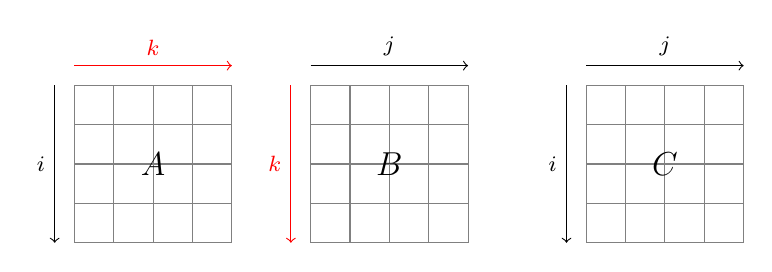
\begin{tikzpicture} [font=\footnotesize]
		\draw [step=.5cm,gray] (-1,-1) grid (1,1);
		\draw [step=.5cm,gray] (1.9999,-1) grid (4,1);
		\draw [step=.5cm,gray] (5.4999,-1) grid (7.5,1);
		
		\node [font=\large] at (0,0) {$A$};
		\node [font=\large] at (3,0) {$B$};
		\node [font=\large] at (6.5,0) {$C$};
		
		\draw [->] (-1.25,1) -- (-1.25,-1) node [midway,left] {$i$};
		\draw [->,red] (-1,1.25) -- (1,1.25) node [midway,above,color=red] {$k$};
		\draw [->,red] (1.75,1) -- (1.75,-1) node [midway,left,color=red] {$k$};
		\draw [->] (2,1.25) -- (4,1.25) node [midway,above] {$j$};
		
		\draw [->] (5.25,1) -- (5.25,-1) node [midway,left] {$i$};
		\draw [->] (5.5,1.25) -- (7.5,1.25) node [midway,above] {$j$};
	\end{tikzpicture}
	
	%\begin{program}
%\FOR i:=1 \TO n \DO
%   \FOR j:=1 \TO n \DO
 %     c_{ij}:=0
 %     \FOR k:=1 \TO n \DO
 %        c_{ij}:=c_{ij} + a_{ik}*b_{kj};
%      \OD
%   \OD
%\OD
	%\end{program}
	
%	\begin{displaymath}
%	for i:=0; i<n; i++)
%	   for(j=0; j<n; j++) {
%	   
%	      c[i][j] = 0;
%	      
%	      for(k=0; k<n; k++)
%	         c[i][j] += a[i][k] * b[k][j];
%	   }
%	   \end{displaymath}
\end{frame}

\begin{frame} [fragile] \frametitle{Matrixmultiplikation 2}
	\begin{enumerate} \setcounter{enumi}{1}
	\item $C=A \cdot B \Leftrightarrow C=A \cdot B'^T$ mit $B'=B^T$
	\par in Pseudocode:
	\begin{lstlisting}[numbers=none, basicstyle=\footnotesize, language=,morekeywords={for, do, to, end},keywordstyle=\color{blue}\underbar]
		         c_ij += a_ik * b'_jk;
	\end{lstlisting}
	Indexreihenfolge IJK-T: $A$ und $B$ zeilenweise durchlaufen
	
	\end{enumerate}
\end{frame}

\begin{frame} [fragile] \frametitle{Matrixmultiplikation 3}
	\begin{enumerate} \setcounter{enumi}{2}
	\item Blocking
	\begin{itemize}
	\item eindimensional: K-blocked IKJ
	
	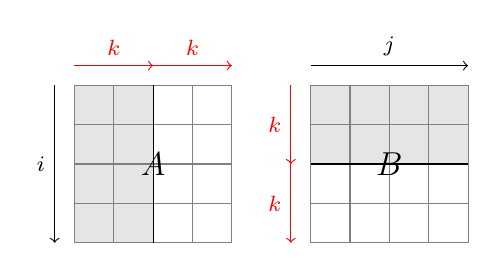
\begin{tikzpicture} [font=\footnotesize]
		\fill [gray!20] (-1,-1) rectangle +(1,2);
		\draw [step=.5cm,gray] (-1,-1) grid (1,1);
		\fill [gray!20] (2,0) rectangle +(2,1);
		\draw [step=.5cm,gray] (1.9999,-1) grid (4,1);
		
		\draw (0,1) -- (0,-1);
		\draw (2,0) -- (4,0);
		
		\node [font=\large] at (0,0) {$A$};
		\node [font=\large] at (3,0) {$B$};
		
		\draw [->] (-1.25,1) -- (-1.25,-1) node [midway,left] {$i$};
		\draw [->,red] (-1,1.25) -- (0,1.25) node [midway,above,color=red] {$k$};
		\draw [->,red] (0,1.25) -- (1,1.25) node [midway,above,color=red] {$k$};
		\draw [->,red] (1.75,1) -- (1.75,0) node [midway,left,color=red] {$k$};
		\draw [->,red] (1.75,0) -- (1.75,-1) node [midway,left,color=red] {$k$};
		\draw [->] (2,1.25) -- (4,1.25) node [midway,above] {$j$};
	\end{tikzpicture}
	
	\item zweidimensional: K/J-blocked IKJ
	
	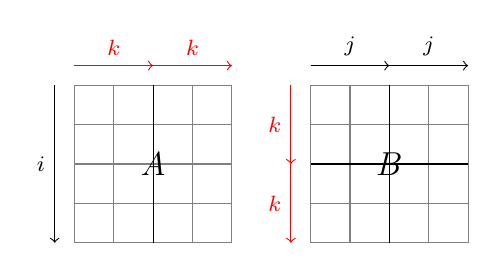
\begin{tikzpicture} [font=\footnotesize]
		\draw [step=.5cm,gray] (-1,-1) grid (1,1);
		\draw [step=.5cm,gray] (1.9999,-1) grid (4,1);
		
		\draw (0,1) -- (0,-1);
		\draw (2,0) -- (4,0);
		\draw (3,1) -- (3,-1);
		
		\node [font=\large] at (0,0) {$A$};
		\node [font=\large] at (3,0) {$B$};
		
		\draw [->] (-1.25,1) -- (-1.25,-1) node [midway,left] {$i$};
		\draw [->,red] (-1,1.25) -- (0,1.25) node [midway,above,color=red] {$k$};
		\draw [->,red] (0,1.25) -- (1,1.25) node [midway,above,color=red] {$k$};
		\draw [->,red] (1.75,1) -- (1.75,0) node [midway,left,color=red] {$k$};
		\draw [->,red] (1.75,0) -- (1.75,-1) node [midway,left,color=red] {$k$};
		\draw [->] (2,1.25) -- (3,1.25) node [midway,above] {$j$};
		\draw [->] (3,1.25) -- (4,1.25) node [midway,above] {$j$};
	\end{tikzpicture}
	
	\end{itemize}
	
	\end{enumerate}
\end{frame}

% Implementierung

\begin{frame} [fragile] \frametitle{Implementierung}
	\begin{itemize}
	
	\item Ziel: flexibler Aufruf von austauschbaren Versionen der Matrixmultiplikation
	
	\item<2-> Signatur:
	\begin{lstlisting}[numbers=none]
	void mm_ijk(int sz,
	            double a[sz][sz], double b[sz][sz], double c[sz][sz])
	\end{lstlisting}
	
	\item<2-> Definition eines Funktionszeigers:
	\begin{lstlisting}[numbers=none]
	typedef void (*mulfunc)(int sz,
                        double a[sz][sz], double b[sz][sz],
                        double c[sz][sz]);
	\end{lstlisting}
	
	\end{itemize}
\end{frame}

\begin{frame} [fragile] \frametitle{Aufruf einer Multiplikationsversion 1}
	Versionsbezeichner:
%	\begin{columns}
%	\begin{column}{4cm}
		\begin{lstlisting}
		struct _mmversion
		{
		   const char* name;
		   mulfunc func;
		} mmversion[] =
		{
		{ "IJK", mm_ijk },
		{ "IJK-T", mm_ijk_t },
		{ "IKJ", mm_ikj },
		{ "JIK", mm_jik },
		{ "JKI", mm_jki },
		{ "KIJ", mm_kij },
		{ "KJI", mm_kji },
		{ "B-IKJ", mm_b_ikj },
		{ "B-KIJ", mm_b_kij },
		{ "BB-IKJ", mm_bb_ikj },
		{ 0,0 }
		};
		\end{lstlisting}
%	\end{column}
	
%	\begin{column}{5cm}
%		Codierung durch Index
%	\end{column}
%	\end{columns}
\end{frame}

\begin{frame} [fragile] \frametitle{Aufruf einer Multiplikationsversion 2}
	\begin{lstlisting}
	void run_mul(mulfunc f, const char* name,
             int sz, double a[sz][sz], double b[sz][sz],
             double c[sz][sz])
{
	   double start, stop, mflops;

	   SSIM_FLUSH_CACHE;
	   
	   start = gettime();
	   
	   init(sz, c, 0);
	   (*f)(sz, a, b, c);
	   
	   stop = gettime();
	   mflops = 2.0*sz*sz*sz / (stop-start) / 1000000.0;
	   
	   fprintf(stderr, "  %s: %f sec. : %f MFlops\n", 
	           name, stop - start, mflops);
	   printf("%f ", mflops);
}
	\end{lstlisting}
\end{frame}

\begin{frame} [fragile] \frametitle{Tracing: Valgrind Client Requests}
	\begin{itemize}
	
	\item Cache leeren:
	\begin{lstlisting}[numbers=none]
	SSIM_FLUSH_CACHE;
	\end{lstlisting}
	
	\item<2-> Speicherzugriffe verfolgen:
	\begin{lstlisting}[numbers=none]
	SSIM_MATRIX_TRACING_START(addr, m, n, ele_size, name);
	\end{lstlisting}
	\begin{itemize}
		\item \verb|addr|: Pointer auf Speicherbereich
		\item \verb|m|, \verb|n|: Matrixdimensionen
		\item \verb|ele_size|: Gr"o"se eines Matrixeintrags
		\item \verb|name|: (eindeutiger) Identifier
	\end{itemize}
	
	\begin{lstlisting}[numbers=none]
	SSIM_MATRIX_TRACING_STOP(addr);
	\end{lstlisting}
	
	\end{itemize}
\end{frame}

\begin{frame} [fragile] \frametitle{Tracing}
	\begin{lstlisting}
	void run_version(int v, int sz, double a[sz][sz], double b[sz][sz], 
	                 double c[sz][sz])
	{
	   const int len = 256;
	   char name[len];
	   
	   strcpy(name + strlen(mmversion[v].name), " - a");
	   SSIM_MATRIX_TRACING_START(a, sz, sz, sizeof(double), name);

	   strcpy(name + strlen(mmversion[v].name), " - b");
	   SSIM_MATRIX_TRACING_START(b, sz, sz, sizeof(double), name);

	   strcpy(name + strlen(mmversion[v].name), " - c");
	   SSIM_MATRIX_TRACING_START(c, sz, sz, sizeof(double), name);

	   run_mul(mmversion[v].func, mmversion[v].name, sz, a, b, c);

	   SSIM_MATRIX_TRACING_STOP(a);
	   SSIM_MATRIX_TRACING_STOP(b);
	   SSIM_MATRIX_TRACING_STOP(c);
	}
	\end{lstlisting}
\end{frame}

\begin{frame} [fragile] \frametitle{Weitere Details}
	\begin{columns}
		\begin{column}{2.75cm}
		\begin{tikzpicture} [font=\footnotesize,rect/.style={rounded corners, draw, fill=gray!10}]
		\node [rect] (m) at (0,0) {\texttt{main}};
		\node [rect, below=1.5cm of m] (r) {\texttt{run}} edge [<-] node {f"ur jede Matrixgr"o"se} (m);
		\node [rect, below=1.5cm of r, rectangle split, rectangle split parts=2] (v) {
			\texttt{run\_version}
			\nodepart{second} \texttt{run\_mul}
		} edge [<-] node {f"ur jede Version} (r);
		
		\node [above=0.5cm of m] {\texttt{funcname}, \texttt{sz1}, \texttt{sz2}} edge [->, dashed] (m);
		\end{tikzpicture}
		\end{column}
		
		\begin{column}{9.25cm}
			\begin{itemize}
			\item<2-> \texttt{main}:
			\begin{lstlisting}
			int v;
			for (v=0; mmversion[v].func != 0; v++)
			   if (funcname != 0
			       && strcmp(funcname, mmversion[v].name)== 0) 
			       break;
			       
			/* Berechnung von sz aus sz1 und sz2 */
			   run (v, sz);
			\end{lstlisting}
			
			\item<3-> \texttt{run(int v, int sz)}:
			\begin{lstlisting}
			if (mmversion[v].func != 0)
			   run_version(v, sz, *a, *b, *c);
			else
			   for(v=0; mmversion[v].func != 0; v++)
			      run_version(v, sz, *a, *b, *c);
			\end{lstlisting}
			\end{itemize}
		\end{column}
	\end{columns}
\end{frame}

